% The two lines of optimizers that merge into Adam. TikZ: a still structure diagram (boxes and arrows).
% Our own drawing of the Note's section 3; the update rules are those of Notes 1034-1038.
\documentclass[tikz,border=8pt]{standalone}
% Shared look for every TikZ diagram. Load with \input{../../tools/tikz-style.tex}
\usepackage[T1]{fontenc}
\usepackage{lmodern}
\renewcommand{\sfdefault}{lmr}  % diagrams use the same serif as the text
\usetikzlibrary{arrows.meta, positioning, shapes.geometric, calc, fit, backgrounds}
\definecolor{cblue}{HTML}{4C78A8}
\definecolor{corange}{HTML}{F58518}
\definecolor{cgreen}{HTML}{54A24B}
\definecolor{cred}{HTML}{E45756}
\definecolor{cpurple}{HTML}{B279A2}
\definecolor{cgrey}{HTML}{6B6B6B}
\tikzset{
  every picture/.style={font=\sffamily, line width=1.2pt},
  box/.style={draw=#1, fill=#1!12, rounded corners=4pt, align=center, inner sep=7pt, minimum height=1.1cm},
  box/.default=cgrey,
  arrow/.style={-{Stealth[length=3mm]}, draw=cgrey, line width=1.4pt},
  title/.style={font=\sffamily\bfseries\Large},
  note/.style={font=\sffamily\small, text=cgrey, align=center},
}
\AtBeginDocument{\hyphenpenalty=10000 \exhyphenpenalty=10000}

\begin{document}
\begin{tikzpicture}[every node/.append style={font=\sffamily},
  opt/.style={draw=#1, line width=1.2pt, rounded corners=4pt, fill=#1!10, align=center, minimum width=4.6cm, minimum height=1.5cm, inner sep=5pt}]
  \node[opt=cgrey] (gd) at (0,0) {\textbf{Gradient descent}\\ $w \leftarrow w - \eta\, g$};
  % idea 1
  \node[font=\sffamily\bfseries, text=cblue, align=center] at (-5.2,-1.25) {Idea 1:\\ speed from past gradients};
  \node[opt=cblue] (mom) at (-3.4,-3.0) {\textbf{Momentum}\\ average of past gradients};
  \node[opt=cblue] (nag) at (-3.4,-5.4) {\textbf{NAG}\\ momentum + look ahead};
  % idea 2
  \node[font=\sffamily\bfseries, text=corange, align=center] at (5.2,-1.25) {Idea 2:\\ a learning rate per parameter};
  \node[opt=corange] (ada) at (3.4,-3.0) {\textbf{AdaGrad}\\ divide by $\sqrt{\text{sum of } g^2}$};
  \node[opt=corange] (rms) at (3.4,-5.4) {\textbf{RMSProp}\\ divide by $\sqrt{\text{average of } g^2}$};
  % adam
  \node[opt=cgreen, minimum width=10cm] (adam) at (0,-8.2) {\textbf{Adam}\\ $w \leftarrow w - \eta\,\dfrac{\hat m}{\sqrt{\hat v}+\epsilon}$\\[2pt]
     {\color{cblue}$\hat m$: average of gradients}\quad {\color{corange}$\hat v$: average of $g^2$}\\ both corrected for starting at 0};
  \draw[arrow] (gd.south) -- ++(0,-0.35) -| (mom.north);
  \draw[arrow] (gd.south) -- ++(0,-0.35) -| (ada.north);
  \draw[arrow] (mom) -- (nag);
  \draw[arrow] (ada) -- (rms);
  \draw[arrow, cblue, line width=1.4pt] (mom.west) -- ++(-0.5,0) |- (adam.west);
  \draw[arrow, corange, line width=1.4pt] (rms.south) -- (rms.south |- adam.north);
\end{tikzpicture}
\end{document}
